%\documentclass[11pt]{article}
\documentclass{report}
\usepackage[nottoc,notlot,notlof]{tocbibind}
\usepackage[english]{babel}
\usepackage{graphicx}
\usepackage{setspace}
\usepackage{subcaption}
\usepackage{enumerate}
\usepackage[export]{adjustbox}
\setstretch{1.5}
\usepackage{url}
\usepackage[title,titletoc,toc]{appendix}
\usepackage[font=small,labelfont=bf,justification=raggedright,singlelinecheck=false]{caption}
%%%%%%%%%% Start TeXmacs macros
\setlength{\voffset}{0.3in}
\setlength{\textheight}{8.5in}
\setlength{\topmargin}{-0.5in}
\setlength{\headheight}{0.0in}
\setlength{\headsep}{-0.0in}
\setlength{\footskip}{0.8in}
\flushbottom
\setlength{\textwidth}{5.6in}
\setlength{\oddsidemargin}{0.5in}
\setlength{\evensidemargin}{0.5in}
\setlength{\columnsep}{2pc}
\setlength{\parindent}{1em}
%%%%%%%%%% End TeXmacs macros

\usepackage{authblk}
\usepackage{hyperref}
\usepackage{refstyle}

\begin{document}
\title{CS 6630: Project Process Book
	\\TED talks topic trend visualization\\}
\author{Hsuan Lee}
\author{Chien-Wei Sun}
\affil{School of Computing, University of Utah}

\maketitle

\tableofcontents{}
\chapter{Overview}
\section{Overview and Motivation}

\quad TED is a leading organization which provides influential and understandable talk to the world. These talks cover a lot of fields, from anthropology to machine learning, and also from biology to sociology. We are interested in the relationship between technology and world market, and we want to know if TED somehow shows the trend of popular technology or it provides a platform for topics which do not get much attention in the world. 

\quad The relevance of different categories is also what we want to discover. For example, several years ago, it was popular that researchers tried to innovate theory according to the behavior of insects, like ants and bees. There are many theories developped based on the cooperation pattern of those animals. In the past, people did not consider that there is a strong relevence between insects and learning theory. We also wonder if we can find situation which is similar to the example.

\section{Related Work}

\quad When we are searching useful data for this project, we found the TED talks dataset and also a visulization by Sean Miller\cite{prework}. In this visualization, it shows statistics of the dataset and also allow user to search video by one tag. However, this visualization does not answer the questions we mention in the above. That's why we decide to build our own visualization of the dataset.


\section{Questions}
\quad Here are questions we expect to answer at the end of this project:
\begin{itemize}
\item
What are the trend of category tags appeared on TED talks?
\item
Is there any relationship between the TED talks and the big events happened in the world? 
\item
Is there a strong relevence between two topics that in general people will not think they are related?
\item
Can we learn the trend of research on a specific field by analyzing the popularity of keywords? Or it shows the topics which people do not put attention on for now but will become important in the future?
\end{itemize}

\chapter{Data}
\section{Dataset}

\quad We find the dataset from Dataset Distribution Portal\cite{idiap}.
This dataset include the video recording from the TED website from 1972 to 2017. For each video, its data contains the following attributes:{}
\begin{figure} [h]
\begin{center}
\includegraphics[scale=0.4]{"csv"}
\caption{Data get from idiap.ch}
\label{fig:csv}
\end{center}
\end{figure}

\begin{center}
\begin{tabular}{l|l}
id & month filmed \\
Speaker & year filmed\\
headline & event\\
URL & duration \\
description & date published \\
transcript URL  & tags \\ 
 \end{tabular}
\end{center}

%\clearpage

\quad To better understand the impact of TED videos, we develop web crawlers to collect attributes like \textbf{rates}(how do people feel after watching a video), \textbf{views}(how many time a video has been played), and some potentially valuable data like datetime, redirected urls, and transcripts. We use \textbf{Scrapy}\cite{scrapy}  as our crawler. Figure~\ref{fig:ratethistalk} displays the rating options on TED website.

\begin{figure} [h]
\begin{center}
\includegraphics[scale=0.4]{"ratethistalk"}
\caption{How people rate one video in TED website}
\label{fig:ratethistalk}
\end{center}
\end{figure}

Furthermore, in order to load data easily, we transfer our data from csv file to json form. We found this preprocessing can be accomplished painlessly by using  \textbf{Pandas}\cite{pandas} toolkit. Figure~\ref{fig:jsonofvideo} shows what kind of data one video contains.

\begin{figure} [h]
\begin{center}
\includegraphics[scale=0.4]{"onevideodata"}
\caption{Data of one video in JSON}
\label{fig:jsonofvideo}
\end{center}
\end{figure}

\quad We plan to visualize the data according to the tags/keywords of the video. It is not efficient to search all the data to find which videos are related with one specific tag on javascript. For practical implementation, we will preprocess the dataset based on tags, which means to use tag as key to create input data.

\section{Exploratory Data Analysis}

\quad In our design, the main chart user interact with is the network chart, which present the co-occurrence of tags. Hence, after we finish the job of collecting data, we move forward to build the co-occurrence matrix of tags. During this procedure, we observe that some tags appear in too many videos so that their existences are not meaningful to the matrix. These tags are `science', `technology', `global issue'. Since they show up in most of talks, we remove them from the matrix so that the network chart will look clear.

\quad To create groups of tags, we apply k-means to divide them into 11 clusters, and one of them restore the outliers. Figure~\ref{fig:group} are the results of two groups. One is the group whose center is tag `computers', the other is the group whose center is `universe'. Color is used to distinguish the group in our design.
\begin{figure} [h]
\begin{center}
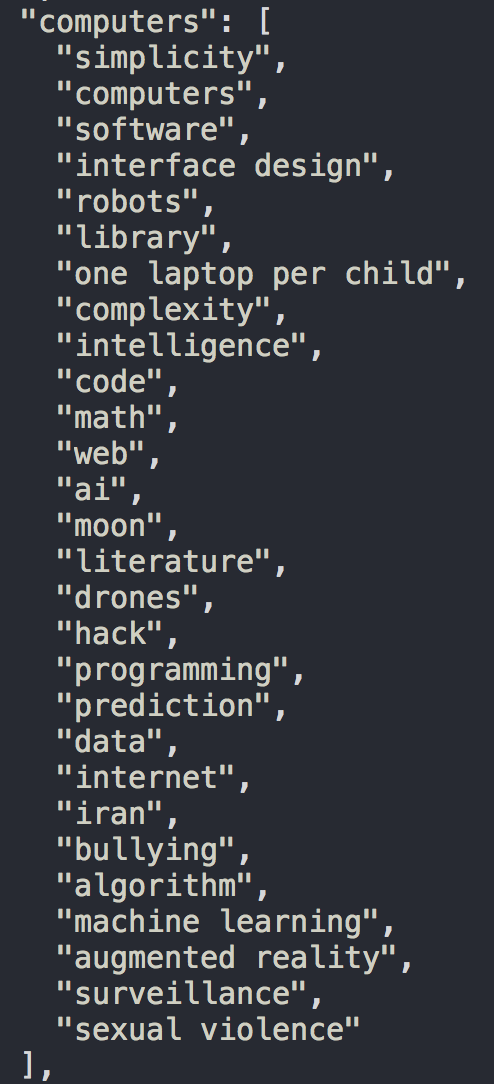
\includegraphics[scale=0.5]{computersgroup}
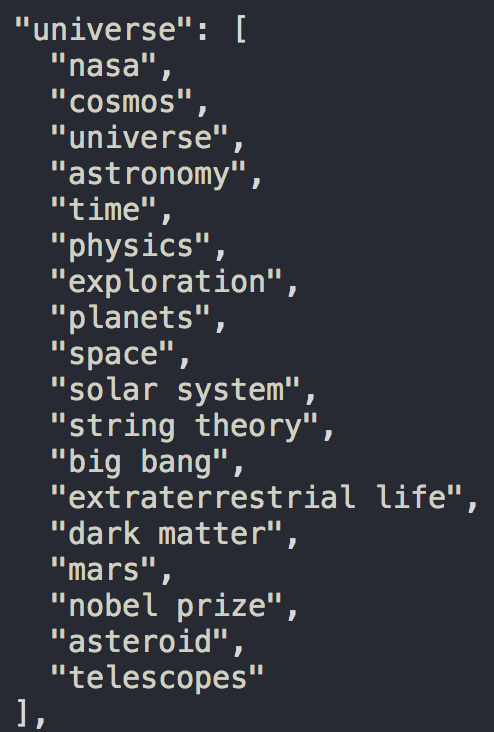
\includegraphics[scale=0.5]{universegroup}
\caption{Clustering result}
\label{fig:group}
\end{center}
\end{figure}
%\clearpage

\chapter{Design Evolution}

\section{Prototype}
\quad Our design is based on the network layout, as shown in Figure~\ref{fig:design1}. This network is composed of tags, and user can choose several tags they are interested in to through interaction with the network node. Next, the line chart in the middle of Figure~\ref{fig:design1} will display the tendency of chosen tags versus time/year. The last part help user to search for TED talks including these tags. User can decide the result is sorted by views or popularity.

\begin{figure} [h]
\begin{center}
\includegraphics[scale=0.13]{"IMG_9010".JPG}
\caption{Category of data, and it relationship with the layout}
\label{fig:design1}
\end{center}
\end{figure}

\begin{figure} [h]
\begin{center}
\includegraphics[scale=0.13]{"IMG_9011".JPG}
\caption{Design of Optional features}
\label{fig:design2}
\end{center}
\end{figure}

\quad We also want to compare the statistic of the tags between years, so we design a bar chart as shown in Figure~\ref{fig:design2}. By making use of the sliding bar on the top, the statistics of two years is displayed. Figure~\ref{fig:data} helps us to figure out what attributes are needed in each chart. It also shows the relationship of charts.  

\begin{figure} [h]
\begin{center}
\includegraphics[scale=0.8]{"Untitled Diagram".png}
\caption{Category of data, and it relationship with the layout}
\label{fig:data}
\end{center}
\end{figure}

\section{Evolution 1}

\quad First, we generate the network chart accoring the co-occurence matrix. Each node represent a tag, and the thickness of one link is decided by the co-occurence value between two tags. However, there are 403 tags and 19488 links on this chart, which make the network look crazy and take a lot of time to draw these lines, as shown in Figure~\ref{fig:networkball}. 

\quad We discuss how to fix this issue and propose two solution for that. One is to draw chord layout in the beginning. Chord layout help people understand the relationship between two groups. We can let user to click ribbon to then show the network layout of tags in these two groups. However, this design does not allow us to observe all the related tags of one tag we choose. The other solution is to reduce the amount of links and nodes. We can provide an overview of network chart with nodes and links whose frequencies and value of co-occurence are bigger than threshold. Then, to zoom in on this chart, user can double-click on the tag they interested in to find all the other tag which is related to the chosen one. After applying the second method, our network chart looks better, as you can find in Figure~\ref{fig:networkwithcolor}.
\begin{figure} [h]
\begin{center}
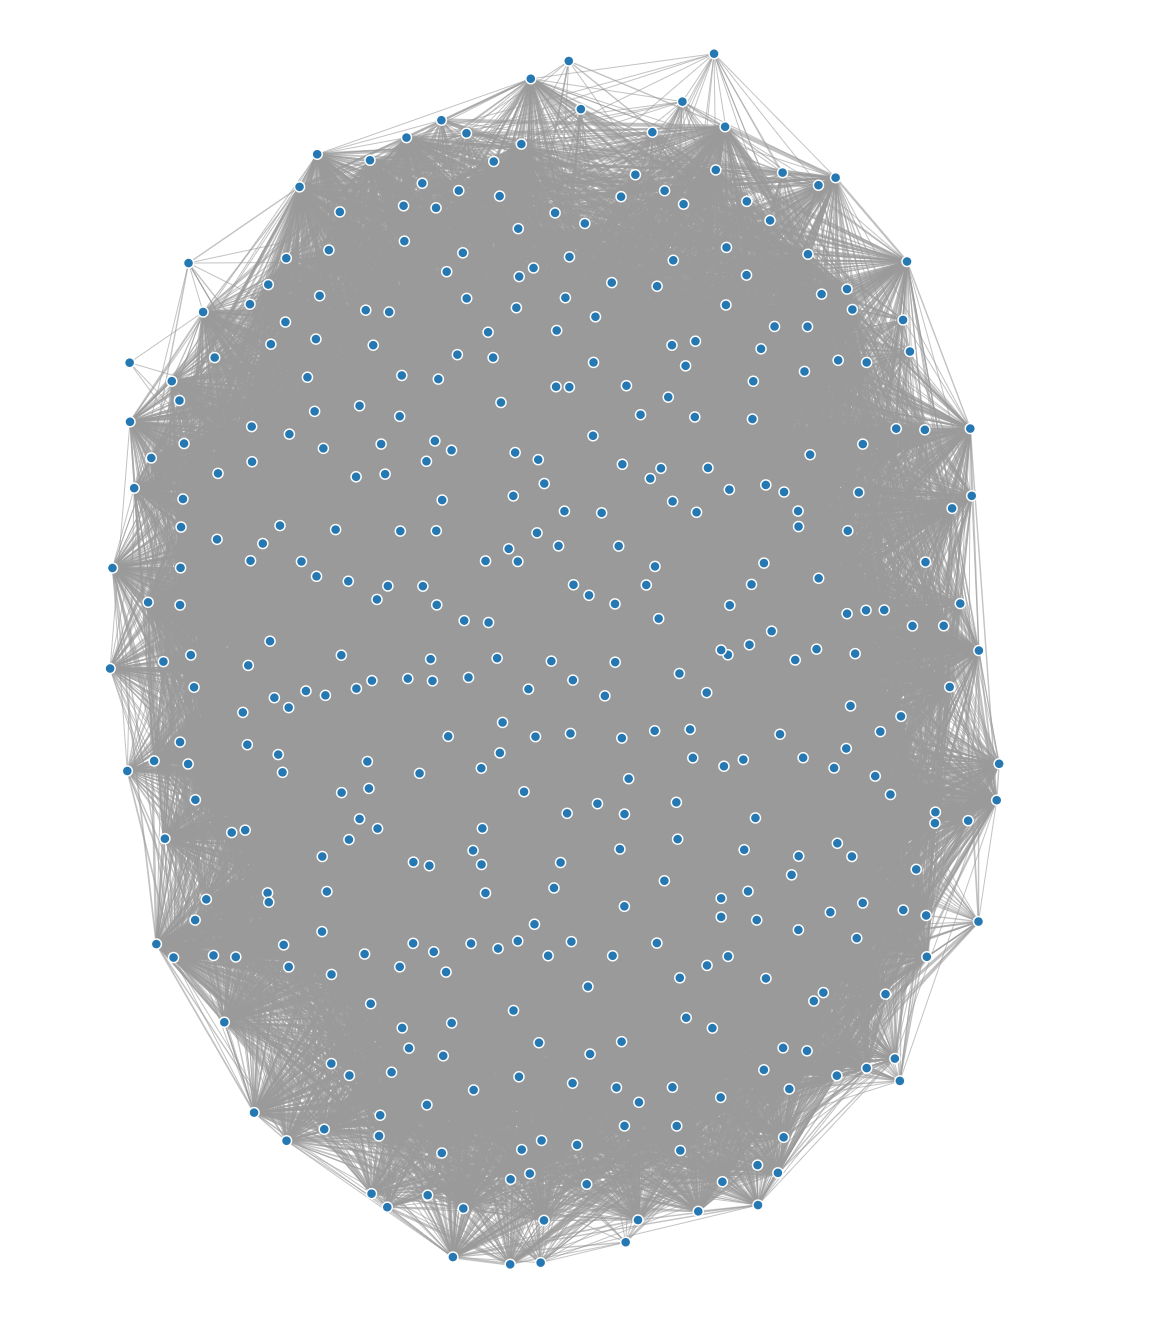
\includegraphics[scale=0.3]{Crazylink}
\caption{Network chart with Over 19,000 links}
\label{fig:networkball}
\end{center}
\end{figure}

\begin{figure} [h]
\begin{center}
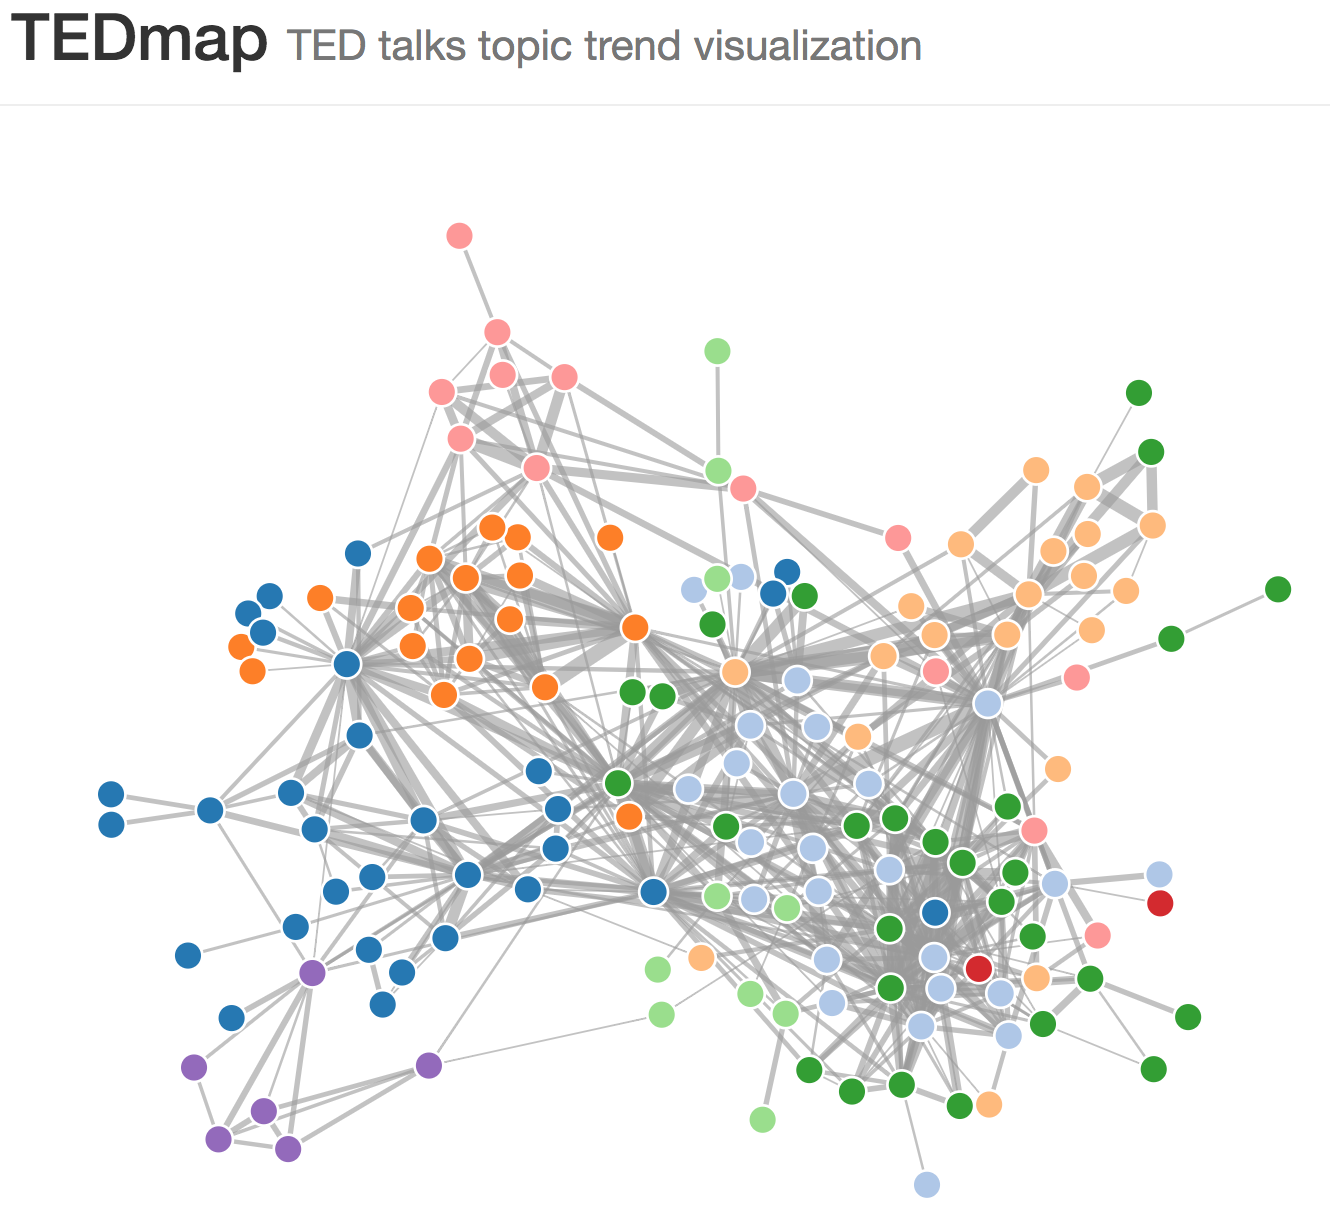
\includegraphics[scale=0.5]{networkChartProto}
\caption{Network chart with link vale bigger than 15}
\label{fig:networkwithcolor}
\end{center}
\end{figure}	


%\appendix


\bibliographystyle{acm}
%%\bibliography{nfv.bib}
\bibliography{js6.bib}

\end{document}
